\documentclass[10pt]{article}
\usepackage{dfsha-informe}

\hito{4}
\title{DFSha: Informe final}
\date{24 de octubre de 2026}

\begin{document}
\portada

\textbf{Opción asignada:} Opción 1, Cliente/Servidor, con el servicio distribuido entre varios nodos dentro de una red privada.

Este es el informe técnico final del proyecto. Reúne lo que se especificó en el Hito 1 y se construyó en el Hito 2, y describe lo que se agregó para cubrir el Hito 3 (alta disponibilidad, replicación, consistencia y seguridad) y la entrega final. Como en los informes anteriores, las decisiones se enuncian en el cuerpo y se justifican en las \textbf{Notas} del final. Las notas de otros hitos se citan como \emph{Hito 1, N3}.

\textbf{Código fuente:} \url{https://github.com/AndresVelezR/DFSha---Distributed-Systems}.

\separador

% =============================================================================
\section{1. Objetivo, problema y marco teórico}

\subsection{Objetivo}

Diseñar e implementar un sistema de archivos distribuido que guarde archivos grandes repartidos entre varios nodos, con escritura y lectura distribuidas, y que siga funcionando sin perder datos cuando falla una máquina. Todo con las comunicaciones y el almacenamiento cifrados, control de acceso por usuario y ubicación dinámica de los datos.

\subsection{Problema}

Un solo servidor de archivos es a la vez el límite de capacidad, el cuello de botella de la red y un punto único de falla: si se cae, no hay servicio, y si pierde su disco, se pierden los archivos. Repartir los archivos entre varias máquinas resuelve la capacidad y el rendimiento, pero trae tres problemas nuevos. Hay que saber en todo momento dónde está cada pedazo de cada archivo, y esa información no se puede perder. Hay que mantener varias copias sin que diverjan. Y hay que decidir qué hacer cuando una máquina deja de responder en la mitad de una operación.

\subsection{Marco teórico}

Un sistema de archivos distribuido guarda archivos repartidos en varias máquinas y los presenta como un solo árbol de directorios. Hay dos enfoques. En el almacenamiento por objetos, como S3, la unidad es el archivo completo. En el almacenamiento por bloques, como GFS y HDFS, el archivo se parte y cada parte se ubica por separado. DFSha es por bloques porque el enunciado pide que cada archivo quede repartido entre varios nodos y que haya concurrencia dentro de un mismo archivo (Hito 1, N1).

De GFS y HDFS se toman dos ideas. La primera es separar el plano de control del plano de datos: un nodo coordinador guarda solo metadatos y decide dónde va cada bloque, y los bytes viajan directamente entre el cliente y los nodos de almacenamiento. La segunda es la escritura única: un bloque guardado no se modifica nunca, así que dos copias del mismo bloque son idénticas por construcción.

El coordinador no puede ser una sola máquina, porque sin él nadie sabe dónde está nada. Replicarlo exige que todas sus copias apliquen los mismos cambios en el mismo orden, aunque algunas se caigan o se desconecten. Ese es el problema del \textbf{consenso}, y DFSha lo resuelve con \textbf{Raft} \vernota{N1}. En Raft, las réplicas eligen un líder. El líder recibe cada cambio, lo agrega a un registro y lo replica a las demás. Un cambio se considera confirmado cuando una mayoría lo guardó en disco. Con tres réplicas la mayoría es dos, así que el sistema tolera la caída de una cualquiera, y nunca puede haber dos líderes aceptando cambios a la vez, porque cada uno necesitaría su propia mayoría.

Para la seguridad se usan piezas estándar: TLS para cifrar las comunicaciones, AES-256-GCM para cifrar y autenticar los bloques en disco, bcrypt para guardar contraseñas y HMAC-SHA256 para firmar los permisos que emite el sistema.

\separador

% =============================================================================
\section{2. Descripción del servicio}

DFSha guarda archivos de cualquier tipo partiéndolos en bloques que se reparten y se replican entre servidores, y los recupera reconstruyéndolos a partir de esos bloques. Un archivo grande nunca se guarda completo en una sola máquina ni se carga completo en memoria.

\subsection{Componentes}

\begin{itemize}
\item \textbf{Cliente} (Python, sin dependencias externas). Programa de línea de comandos que también se puede usar como biblioteca. Se autentica, ejecuta los comandos, parte los archivos al subirlos y los reconstruye al bajarlos. No es parte del servicio.
\item \textbf{ControlNode} (Go). Hay tres. Guardan los metadatos: el árbol de directorios de cada usuario, qué bloques forman cada archivo y dónde está cada copia. Uno de ellos es el líder: atiende al cliente, calcula los planes de subida y bajada, y repara y rebalancea las copias. No guarda datos de archivos.
\item \textbf{DataNode} (Go). Tres o más. Guardan los bloques cifrados en su disco, los entregan completos o por rangos y los copian a otros DataNodes cuando el líder lo ordena.
\end{itemize}

\subsection{Operaciones del cliente}

\begin{xltabular}{\linewidth}{@{}L{2.6cm}L{5.4cm}Y@{}}
\toprule
Requisito & Comandos & Qué hacen \\
\midrule\endhead
RF1, gestión & \texttt{ls}, \texttt{cd}, \texttt{pwd}, \texttt{mkdir}, \texttt{rmdir}, \texttt{rm}, \texttt{mv}, \texttt{stat} & Recorren y cambian el árbol del usuario. Solo tocan metadatos. \texttt{stat} muestra tamaño, bloques y en qué DataNodes está cada copia \\
RF2, transferencia & \texttt{put} o \texttt{send}, \texttt{get} o \texttt{receive} & Suben y bajan un archivo completo, con varios bloques en paralelo \\
RF3, acceso & \texttt{open}, \texttt{lock}, \texttt{read}, \texttt{write}, \texttt{close} & Abren un archivo y devuelven un identificador (\emph{handle}); leen un rango de bytes descargando solo los bloques que lo contienen; reservan el archivo para un solo escritor; escriben bytes desde una posición publicando una versión nueva \\
Clúster & \texttt{status} & Muestra los DataNodes, su ocupación y el estado de Raft \\
\bottomrule
\end{xltabular}

\subsection{Cómo se cubren los requisitos no funcionales}

\begin{xltabular}{\linewidth}{@{}L{3.2cm}Y@{}}
\toprule
Requisito & Cómo se cubre \\
\midrule\endhead
RNF1, escalabilidad & Los DataNodes se agregan con el sistema en marcha: un nodo nuevo solo arranca y se registra, y empieza a recibir bloques. El tamaño de bloque se adapta al número de nodos y los ControlNodes solo guardan metadatos (secciones 5 y 9) \\
RNF2, disponibilidad & Tres ControlNodes con Raft toleran la caída de uno. Cada bloque tiene dos copias en DataNodes distintos, y el líder repone las que se pierden (sección 6) \\
RNF3, consistencia & Bloques inmutables identificados por su SHA-256, metadatos replicados por mayoría, un solo escritor por archivo y publicación atómica (sección 7) \\
RNF4, particionamiento & Todo archivo se parte en bloques repartidos entre DataNodes, y las copias de un mismo bloque nunca quedan en el mismo nodo (sección 5) \\
RNF5, rendimiento & El cliente transfiere varios bloques a la vez contra DataNodes distintos, y cada DataNode atiende varias peticiones en paralelo (secciones 5 y 10) \\
RNF6, seguridad & HTTPS en todos los canales y TLS mutuo entre ControlNodes, bloques cifrados en disco, usuarios con contraseña, árbol privado por usuario y permisos firmados para cada acceso a un bloque (sección 8) \\
RNF7, transparencia & El cliente no conoce ningún DataNode de antemano: recibe sus direcciones en cada plan, y si un ControlNode no es el líder, le indica cuál es. El usuario solo ve rutas \\
\bottomrule
\end{xltabular}

\subsection{Fuera del alcance}

No se monta como unidad del sistema operativo: el acceso es por línea de comandos y API. No hay permisos compartidos entre usuarios ni grupos: cada usuario ve solo su árbol \vernota{N9}. El número de ControlNodes es fijo en tres.

\separador

% =============================================================================
\section{3. Arquitectura}

\textbf{Tipo de arquitectura: Maestro y Trabajador, con el maestro replicado.} Los ControlNodes coordinan y saben dónde está todo, y los DataNodes guardan los datos. A diferencia del Hito 2, el maestro ya no es una sola máquina sino un grupo de tres que se mantiene igual con Raft.

\begin{figure}[htbp]
\centering
\begin{tikzpicture}
  \node[caja, minimum width=2.4cm] (cli) at (0,-3.0) {Cliente\\\footnotesize CLI en Python};
  \node[caja, minimum width=3.0cm] (cn1) at (6.6,1.4) {ControlNode cn-01\\\footnotesize líder};
  \node[caja, minimum width=2.4cm] (cn2) at (10.4,2.2) {cn-02\\\footnotesize seguidor};
  \node[caja, minimum width=2.4cm] (cn3) at (10.4,0.6) {cn-03\\\footnotesize seguidor};
  \node[caja, minimum width=3.0cm] (dn1) at (6.6,-1.6) {DataNode dn-01};
  \node[caja, minimum width=3.0cm] (dn2) at (6.6,-2.8) {DataNode dn-02};
  \node[caja, minimum width=3.0cm] (dn3) at (6.6,-4.0) {DataNode dn-03};
  \node[cajaclara, minimum width=3.0cm] (dn4) at (6.6,-5.2) {DataNode dn-04\\\footnotesize se agrega en caliente};
  \coordinate (espacio) at ($(dn2.east)+(1.4,0)$);
  \node[draw, gray!60, rounded corners=3pt, inner sep=7pt, fit=(dn1)(dn4)(espacio)] (dns) {};

  \draw[flecha] (cli.north) |- node[pos=0.75, above, font=\footnotesize] {HTTPS: planes y metadatos} (cn1.west);
  \draw[flecha] (cli.east) -- node[above, sloped, font=\footnotesize] {HTTPS: bloques} (dn1.west);
  \draw[flecha] (cli.east) -- (dn2.west);
  \draw[flecha] (cli.east) -- (dn3.west);
  \draw[flechaclara] (cli.east) -- (dn4.west);
  \draw[flecha, <->] (cn1.east) -- (cn2.west);
  \draw[flecha, <->] (cn1.east) -- (cn3.west);
  \node[font=\footnotesize, align=center] at (12.6,1.4) {Raft\\TLS mutuo};
  \draw[flecha] (dns.north) -- node[right, font=\footnotesize, align=left] {heartbeat\\e inventario} (cn1.south);
  \draw[flecha] (dn1.east) to[bend left=55] (dn2.east);
  \draw[flecha] (dn2.east) to[bend left=55] node[right, font=\footnotesize, align=left] {copias entre\\DataNodes} (dn3.east);
\end{tikzpicture}
\caption{Componentes y comunicaciones. Los bloques nunca pasan por los ControlNodes.}
\end{figure}

\subsection{Plano de control y plano de datos}

El cliente le pregunta al líder qué hacer y le responde un \textbf{plan}: para cada bloque, en qué DataNodes va o de cuáles se lee, con un permiso firmado para cada uno. Con ese plan, el cliente mueve los bloques directamente con los DataNodes. El líder nunca recibe el contenido de un archivo, así que el tamaño de los archivos no lo convierte en cuello de botella.

\subsection{Qué estado se replica y cuál no}

Los ControlNodes guardan dos tipos de estado, y la diferencia es central en el diseño \vernota{N2}:

\begin{itemize}
\item \textbf{Replicado por Raft}: directorios, archivos publicados con su lista de bloques, reservas de subida, handles abiertos y subidas ya confirmadas. Es lo que no se puede perder ni contradecir: si se perdiera, se perderían los archivos aunque sus bloques siguieran en disco. Vive en el registro de Raft en disco y es idéntico en los tres ControlNodes.
\item \textbf{Memoria del nodo}: qué DataNodes están vivos, cuánto ocupa cada uno y qué bloques tiene. Es información que los propios DataNodes vuelven a enviar cada pocos segundos, así que si se pierde se reconstruye sola. Los DataNodes mandan su heartbeat a los tres ControlNodes, de modo que un seguidor que gana una elección ya sabe qué DataNodes están vivos.
\end{itemize}

\subsection{Organización del código}

Cada nodo es un binario independiente. Dentro de cada uno el código se separa en archivos por responsabilidad, como en el Hito 2.

\begin{xltabular}{\linewidth}{@{}L{5.2cm}Y@{}}
\toprule
Archivo & Responsabilidad \\
\midrule\endhead
\texttt{controlnode/consensus.go} & Raft: registro en disco, snapshots, TLS mutuo y la máquina de estados que aplica cada cambio confirmado \\
\texttt{controlnode/server.go} & Estado del servidor, rutas, comprobación de liderazgo y publicación de cambios por Raft \\
\texttt{controlnode/planner.go} & Tamaño de bloque, número de copias y ubicación. Funciones puras, sin HTTP \\
\texttt{controlnode/handlers\_*.go} & Endpoints por tema: autenticación, sistema de archivos, subida, descarga y clúster \\
\texttt{controlnode/maintenance.go} & Reparación, rebalanceo y borrado de bloques sin uso \\
\texttt{datanode/storage.go} & Disco: cifrado, verificación, escritura atómica e inventario \\
\texttt{datanode/handlers.go} & Endpoints de bloques y validación de permisos \\
\texttt{datanode/control\_client.go}, \texttt{peer\_client.go} & Registro y heartbeat hacia los ControlNodes; copias hacia otros DataNodes \\
\texttt{datanode/ownership.go} & Registro de qué cuenta subió cada bloque \\
\texttt{internal/common} & TLS, secretos y permisos firmados, compartidos por ambos nodos \\
\texttt{admin} & Genera la CA, los certificados, las claves y los usuarios \\
\texttt{client/dfsha.py} & Cliente de línea de comandos y API \\
\bottomrule
\end{xltabular}

\separador

% =============================================================================
\section{4. Comunicaciones}

El control viaja en JSON y los bloques como cuerpo binario sin codificar, todo sobre HTTPS (Hito 1, N11). La única excepción es Raft, que usa su propio protocolo binario sobre TCP con TLS mutuo. Cada ControlNode expone su API en el puerto \textbf{8000} y Raft en el \textbf{9000}; cada DataNode expone la suya en el \textbf{8001}.

\subsection{Protocolo por cada relación}

\begin{xltabular}{\linewidth}{@{}L{2.4cm}L{2.0cm}L{2.6cm}L{3.3cm}Y@{}}
\toprule
Relación & Expone & Protocolo & Autenticación & Para qué \\
\midrule\endhead
Cliente y ControlNode & ControlNode & REST/JSON sobre HTTPS & Token de sesión & Login, sistema de archivos, planes, confirmación y estado \\
Cliente y DataNode & DataNode & REST/binario sobre HTTPS & Permiso firmado por bloque y nodo & Subir y bajar bloques, completos o por rango \\
DataNode y DataNode & DataNode & REST/binario sobre HTTPS & Permiso del cliente, o clave del clúster en reparaciones & Propagar la copia al subir y reponer copias \\
ControlNode y DataNode & ambos & REST/JSON sobre HTTPS & Clave del clúster & Registro, heartbeat e inventario; órdenes de copiar, verificar y borrar \\
ControlNode y ControlNode & ControlNode & Raft sobre TCP con TLS mutuo & Certificado del clúster en ambos extremos & Elección de líder y réplica del registro de metadatos \\
\bottomrule
\end{xltabular}

\subsection{API del ControlNode para el cliente}

Todas, salvo \texttt{login} y \texttt{health}, requieren \texttt{Authorization: Bearer} con el token de sesión. Si el nodo que recibe la petición no es el líder, responde \texttt{503} con la URL del líder en el campo \texttt{leader}, y el cliente repite la petición allá.

\begin{xltabular}{\linewidth}{@{}L{3.7cm}YYL{3.0cm}@{}}
\toprule
Operación & Solicitud & Respuesta & Errores \\
\midrule\endhead
\texttt{POST} \ruta{/auth/login} & \texttt{\{username, password\}} & \texttt{200 \{token, expires\_in\}} & \texttt{401} \\
\texttt{GET} \ruta{/fs/ls?path=} & sin cuerpo & \texttt{200 \{entries:[\{name, type, size, blocks, replicas\_ok\}]\}} & \texttt{404} \\
\texttt{POST} \ruta{/fs/mkdir} & \texttt{\{path\}} & \texttt{201} & \texttt{404} sin padre, \texttt{409} ya existe \\
\texttt{DELETE} \ruta{/fs/rmdir?path=} & sin cuerpo & \texttt{204} & \texttt{404}, \texttt{409} no vacío \\
\texttt{DELETE} \ruta{/fs/rm?path=} & sin cuerpo & \texttt{204} & \texttt{404}, \texttt{409} con escritor \\
\texttt{POST} \ruta{/fs/mv} & \texttt{\{src, dst\}} & \texttt{200} & \texttt{404}, \texttt{409} destino existe \\
\texttt{GET} \ruta{/fs/stat?path=} & sin cuerpo & \texttt{200 \{size, sha256, block\_size, blocks:[\{index, block\_id, size, stored\_on\}], replicas\_ok\}} & \texttt{404} \\
\texttt{POST} \ruta{/files/upload/plan} & \texttt{\{path, size, sha256\}} & \texttt{200} plan de escritura & \texttt{404}, \texttt{409} reservado, \texttt{503} sin DataNodes, \texttt{507} no cabe \\
\texttt{POST} \ruta{/files/upload/renew} & \texttt{\{upload\_id\}} & \texttt{200} plan con permisos nuevos & \texttt{410} vencida \\
\texttt{POST} \ruta{/files/upload/commit} & \texttt{\{upload\_id, sha256, blocks:[\{index, block\_id, size\}]\}} & \texttt{200 \{status:"publicado"\}} & \texttt{409} bloque sin copias, \texttt{410} vencida \\
\texttt{POST} \ruta{/files/upload/abort} & \texttt{\{upload\_id\}} & \texttt{204} & \texttt{403} \\
\texttt{GET} \ruta{/files/download/plan?path=} & sin cuerpo & \texttt{200} plan de lectura & \texttt{404}, \texttt{503} bloque sin copias vivas \\
\texttt{POST} \ruta{/files/open}, \ruta{/files/lock} & \texttt{\{path, mode\}} & \texttt{200 \{handle, expires\_at\}} & \texttt{404}, \texttt{409} ya hay escritor \\
\texttt{POST} \ruta{/files/renew}, \ruta{/files/close} & \texttt{\{handle\}} & \texttt{200}, \texttt{204} & \texttt{403}, \texttt{410} \\
\texttt{GET} \ruta{/cluster/status} & sin cuerpo & \texttt{200 \{nodes, files, raft\}} & \\
\texttt{GET} \ruta{/health} & sin autenticación & \texttt{200 \{node\_id, role, leader, alive\_datanodes\}} & \\
\bottomrule
\end{xltabular}

Un plan de escritura de un archivo de 100 MiB en el clúster de tres DataNodes; el identificador y los permisos están abreviados:

\begin{codigo}
POST /files/upload/plan  { "path": "/prueba/original.bin", "size": 104857600, "sha256": "24cd..." }
200 OK
{ "upload_id": "9c1e...", "block_size": 8388608, "n_blocks": 13,
  "expires_at": "2026-10-25T04:30:12Z",
  "blocks": [
    { "index": 0, "targets": [ {"node":"dn-02","url":"https://172.31.0.12:8001","token":"eyJ..."},
                               {"node":"dn-03","url":"https://172.31.0.13:8001","token":"eyJ..."} ] },
    ... ] }
\end{codigo}

\subsection{API interna del ControlNode}

\begin{xltabular}{\linewidth}{@{}L{4.2cm}L{3.2cm}Y@{}}
\toprule
Operación & Quién la usa & Para qué \\
\midrule\endhead
\texttt{POST} \ruta{/cluster/register} & DataNode $\rightarrow$ ControlNode & Alta al arrancar con \texttt{\{node\_id, url, capacity, used\}} \\
\texttt{POST} \ruta{/cluster/heartbeat} & DataNode $\rightarrow$ ControlNode & Señal de vida cada 3 s con los mismos datos. Se envía a los tres ControlNodes \\
\texttt{POST} \ruta{/cluster/blockreport} & DataNode $\rightarrow$ ControlNode & Lista de bloques que tiene el DataNode, cada 30 s \\
\bottomrule
\end{xltabular}

Todas exigen la clave del clúster en la cabecera \texttt{X-Cluster-Key}. Los endpoints \ruta{/cluster/replicate} y \ruta{/cluster/election} que definió el Hito 2 ya no existen: esa comunicación es ahora Raft, en el puerto 9000 \vernota{N1}.

\subsection{API del DataNode}

\begin{xltabular}{\linewidth}{@{}L{3.5cm}L{2.0cm}YYL{2.0cm}@{}}
\toprule
Operación & La usa & Solicitud & Respuesta & Errores \\
\midrule\endhead
\texttt{PUT} \ruta{/blocks/{id}} & Cliente, DataNode & Cuerpo binario y permiso de escritura. \texttt{X-Forward-To} con los otros destinos y sus permisos & \texttt{201} si lo creó, \texttt{200} si ya existía; \texttt{\{block\_id, size, stored\_on\}} & \texttt{401}, \texttt{409} firma no coincide, \texttt{507} \\
\texttt{GET} \ruta{/blocks/{id}} & Cliente & Permiso de lectura y opcionalmente \texttt{Range} & \texttt{200} o \texttt{206}, binario & \texttt{401}, \texttt{404}, \texttt{500} corrupto \\
\texttt{HEAD} \ruta{/blocks/{id}} & ControlNode & Clave del clúster y opcionalmente \texttt{X-Block-Owner} & \texttt{200} con firma y tamaño & \texttt{404} \\
\texttt{POST} \ruta{/blocks/{id}/replicate} & ControlNode & \texttt{\{target:\{node, url\}\}} & \texttt{200}, el bloque quedó en el destino & \texttt{404}, \texttt{502} \\
\texttt{DELETE} \ruta{/blocks/{id}} & ControlNode & Clave del clúster & \texttt{204} & \texttt{401} \\
\texttt{GET} \ruta{/inventory} & ControlNode & Clave del clúster & \texttt{\{blocks, used, capacity\}} & \texttt{401} \\
\texttt{GET} \ruta{/health} & Operación & sin autenticación & \texttt{200 \{node\_id\}} & \\
\bottomrule
\end{xltabular}

El identificador \texttt{id} de un bloque es el SHA-256 de su contenido en hexadecimal.

\subsection{Errores y reintentos}

\begin{xltabular}{\linewidth}{@{}L{5.6cm}Y@{}}
\toprule
Situación & Comportamiento \\
\midrule\endhead
El ControlNode contactado no es el líder & Responde \texttt{503} con la URL del líder y el cliente repite allá \\
No hay líder, durante una elección & El cliente recorre los ControlNodes y vuelve a intentar a los 1, 2 y 4 s. Una elección tarda entre 2 y 4 s \\
Fallo de red al subir un bloque & Hasta 3 reintentos contra el mismo DataNode, a los 1, 2 y 4 s. Si sigue sin responder, el siguiente destino del plan pasa a ser el primero \vernota{N7} \\
Fallo al bajar un bloque, o firma incorrecta & Se pasa de inmediato a la siguiente réplica \\
Error del servidor, como \texttt{409} o \texttt{404} & No se reintenta: es una decisión, no un fallo pasajero \\
La reserva venció antes de confirmar (\texttt{410}) & El cliente pide un plan nuevo y repite la subida una vez \\
\bottomrule
\end{xltabular}

\subsection{Cómo funciona una subida}

\begin{center}
\begin{tikzpicture}
  \participante{0}{-10.3}{Cliente}
  \participante{5.4}{-10.3}{ControlNode líder}
  \participante{9.5}{-10.3}{DataNode A}
  \participante{13.1}{-10.3}{DataNode B}
  \mensaje{0}{5.4}{-1.0}{\texttt{POST /files/upload/plan}}
  \mensaje[flechaclara]{5.4}{0}{-2.0}{plan: tamaño de bloque, destinos\\y un permiso por destino}
  \draw[gray!70, rounded corners=2pt] (-1.4,-2.5) rectangle (14.55,-6.4);
  \node[anchor=north west, font=\footnotesize\itshape, text=gray!70!black, fill=white, inner sep=1pt] at (-1.35,-2.52) {por cada bloque, hasta 4 en paralelo};
  \mensaje{0}{9.5}{-3.4}{\texttt{PUT /blocks/\{sha256\}} con \texttt{X-Forward-To: B}}
  \mensaje{9.5}{13.1}{-4.3}{\texttt{PUT /blocks/\{sha256\}}}
  \mensaje[flechaclara]{13.1}{9.5}{-5.0}{201}
  \mensaje[flechaclara]{9.5}{0}{-5.8}{201 \texttt{stored\_on = [A, B]}}
  \mensaje{0}{5.4}{-7.2}{\texttt{POST /files/upload/commit}}
  \mensaje{5.4}{9.5}{-8.0}{\texttt{HEAD}: ¿lo tienes íntegro?}
  \mensaje{5.4}{13.1}{-8.7}{\texttt{HEAD}}
  \node[anchor=west, font=\footnotesize\itshape, text=gray!70!black, fill=white, inner sep=1pt] at (5.55,-9.2) {publica el manifiesto por Raft};
  \mensaje[flechaclara]{5.4}{0}{-9.9}{200 publicado}
\end{tikzpicture}
\end{center}

\begin{enumerate}
\item El cliente calcula el SHA-256 del archivo y pide un plan con la ruta, el tamaño y la firma.
\item El líder valida la ruta, comprueba que nadie más la esté escribiendo y que el archivo quepa, calcula tamaño de bloque, número de copias y destinos, y reserva la ruta por Raft. El archivo todavía no existe para nadie.
\item El cliente lee cada bloque del disco, calcula su firma y lo envía al primer destino, hasta cuatro a la vez. Mientras sube, renueva la reserva cada 20 s.
\item El primer DataNode verifica la firma, cifra el bloque, lo guarda y lo propaga al siguiente destino, para que el cliente envíe cada bloque una sola vez (Hito 1, N12).
\item El cliente confirma. Antes de publicar, el líder le pregunta a cada DataNode del plan si tiene el bloque íntegro y si fue esta cuenta quien lo subió. Si todo está, publica el manifiesto del archivo por Raft, y desde ese instante el archivo existe completo.
\end{enumerate}

\subsection{Cómo funciona una descarga}

\begin{center}
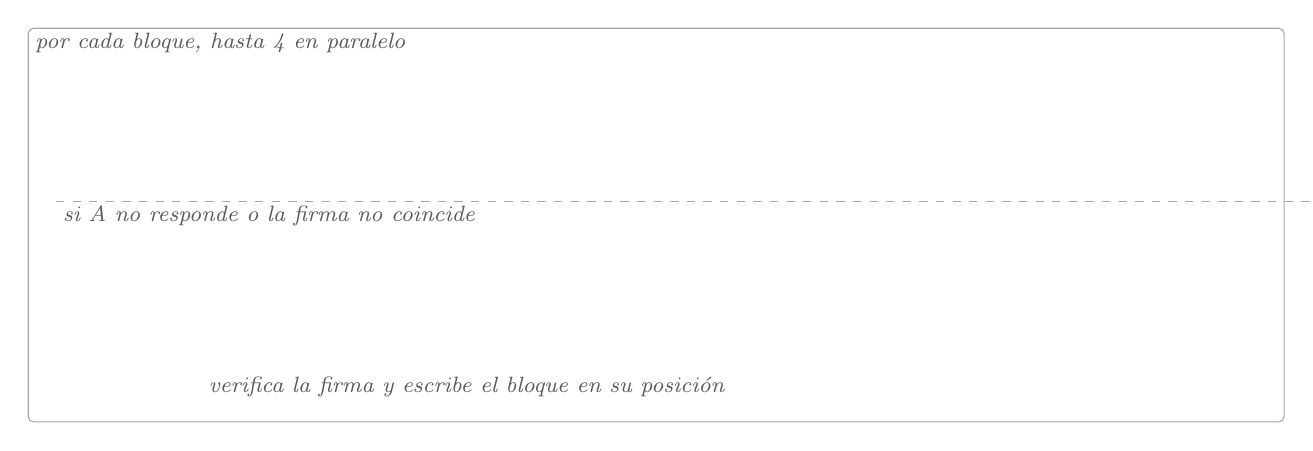
\begin{tikzpicture}
  \participante{0}{-7.9}{Cliente}
  \participante{5.4}{-7.9}{ControlNode líder}
  \participante{9.5}{-7.9}{DataNode A}
  \participante{13.1}{-7.9}{DataNode B}
  \mensaje{0}{5.4}{-1.0}{\texttt{GET /files/download/plan?path=}}
  \mensaje[flechaclara]{5.4}{0}{-2.0}{bloques, réplicas vivas\\y un permiso de lectura por réplica}
  \draw[gray!70, rounded corners=2pt] (-1.4,-2.5) rectangle (14.55,-7.5);
  \node[anchor=north west, font=\footnotesize\itshape, text=gray!70!black, fill=white, inner sep=1pt] at (-1.35,-2.52) {por cada bloque, hasta 4 en paralelo};
  \mensaje{0}{9.5}{-3.4}{\texttt{GET /blocks/\{sha256\}}}
  \mensaje[flechaclara]{9.5}{0}{-4.2}{bloque}
  \draw[gray!70, dashed] (-1.4,-4.7) -- (14.55,-4.7);
  \node[anchor=north west, font=\footnotesize\itshape, text=gray!70!black, fill=white, inner sep=1pt] at (-1.35,-4.72) {si A no responde o la firma no coincide};
  \mensaje{0}{13.1}{-5.6}{\texttt{GET /blocks/\{sha256\}}}
  \mensaje[flechaclara]{13.1}{0}{-6.4}{bloque}
  \node[anchor=west, font=\footnotesize\itshape, text=gray!70!black, fill=white, inner sep=1pt] at (0.15,-7.05) {verifica la firma y escribe el bloque en su posición};
\end{tikzpicture}
\end{center}

Cada bloque verificado se escribe en su posición de un archivo temporal. Al terminar, el cliente compara el SHA-256 del archivo completo con el del manifiesto y solo entonces le da el nombre final. Una descarga fallida nunca deja un archivo que parezca completo.

\separador

% =============================================================================
\section{5. Algoritmos de particionamiento y distribución}

Las decisiones de esta sección viven en \texttt{controlnode/planner.go} como funciones puras y tienen pruebas automáticas.

\subsection{Tamaño de bloque}

Se mantiene la fórmula del Hito 1 (N3):

\begin{codigo}
B = clamp( block_size_min , S / (k · N) , block_size_max )
\end{codigo}

donde \texttt{S} es el tamaño del archivo, \texttt{N} el número de DataNodes vivos y \texttt{k} los bloques mínimos por nodo, redondeando a la potencia de dos inferior. Con los valores por defecto (8 MiB, 64 MiB y \texttt{k = 4}):

\begin{xltabular}{\linewidth}{@{}YYYYY@{}}
\toprule
Archivo & Bloque con 3 nodos & Bloques & Bloque con 4 nodos & Bloques \\
\midrule\endhead
1 MB & 8 MiB & 1 & 8 MiB & 1 \\
100 MiB & 8 MiB & 13 & 8 MiB & 13 \\
500 MB & 32 MiB & 15 & 16 MiB & 30 \\
1 GiB & 64 MiB & 16 & 64 MiB & 16 \\
10 GiB & 64 MiB & 160 & 64 MiB & 160 \\
\bottomrule
\end{xltabular}

Un archivo vacío ocupa un bloque de cero bytes, para que también tenga manifiesto.

\subsection{Número de copias}

Se aplican las dos reglas del Hito 1 (N4): el factor configurado, 2 por defecto, nunca supera \texttt{N - 1} con \texttt{N} el número de DataNodes registrados, y si hay menos DataNodes vivos que ese factor se guardan las copias posibles en vez de rechazar la escritura (Hito 2, N2). Las copias de un mismo bloque siempre quedan en DataNodes distintos.

\subsection{Ubicación de los bloques}

Se usa la asignación voraz al nodo menos cargado, el \emph{list scheduling} de Graham (Hito 1, N5): cada copia de cada bloque va al DataNode vivo con menor porcentaje de ocupación que no tenga ya una copia de ese bloque. Sobre eso, el algoritmo implementado hace cuatro cosas:

\begin{itemize}
\item \textbf{Carga virtual.} Mientras arma el plan, le suma a cada nodo elegido el tamaño del bloque, para que los bloques de una misma subida no caigan todos en los nodos que estaban más vacíos al empezar (Hito 2, N3).
\item \textbf{Reservas en curso.} Antes de empezar, le suma a cada nodo lo que otras subidas todavía en curso ya tienen asignado allí, porque esos bytes aún no aparecen en su disco.
\item \textbf{Umbral de ocupación.} Un nodo no recibe un bloque si con él pasaría de \texttt{FULL\_THRESHOLD\_PERCENT}, 90 \% por defecto. Si algún bloque no consigue todas sus copias, el plan se rechaza con \texttt{507} antes de subir nada.
\item \textbf{Desempate por identificador}, para que el mismo estado produzca siempre el mismo plan.
\end{itemize}

En el clúster de prueba, un archivo de 40 MiB produjo 6 bloques y 12 copias, repartidas exactamente 4, 4 y 4 entre los tres DataNodes, sin ningún bloque con sus dos copias en el mismo nodo.

\subsection{Identificación por contenido}

El identificador de cada bloque es el SHA-256 de su contenido. Eso da tres propiedades sin código adicional: un bloque recibido se puede verificar contra su propio nombre, subir dos veces el mismo bloque no lo duplica, y dos archivos con un bloque idéntico comparten su almacenamiento.

\subsection{Rebalanceo}

Cuando entra un DataNode vacío, las escrituras nuevas lo prefieren de inmediato, porque es el menos ocupado. Si además la diferencia de ocupación entre el nodo más lleno y el más vacío supera el umbral de rebalanceo, 10 \% por defecto, el líder mueve bloques ya guardados, uno por ciclo de mantenimiento, como previó el Hito 1. Cómo se mueve un bloque sin poner en riesgo los datos se explica en la sección 7.

\separador

% =============================================================================
\section{6. Alta disponibilidad}

\subsection{ControlNodes}

Los tres ControlNodes forman un grupo de Raft. Uno es el líder y los otros dos son seguidores que reciben y guardan cada cambio. El líder envía un latido a los seguidores; si un seguidor deja de recibirlo por 2 s, se postula y pide votos, y gana si consigue la mayoría.

\begin{itemize}
\item \textbf{Cae el líder.} En 2 a 4 s los dos que quedan eligen un líder nuevo. Como todo cambio confirmado estaba en al menos dos de los tres registros, y Raft solo deja ganar a un candidato cuyo registro esté al día, el líder nuevo tiene todos los cambios confirmados. El cliente detecta la caída, recorre la lista de ControlNodes y encuentra al nuevo líder.
\item \textbf{Cae un seguidor.} El líder sigue teniendo mayoría con el otro y no se nota nada.
\item \textbf{Caen dos.} El que queda no tiene mayoría y rechaza todas las operaciones con \texttt{503}. Es lo correcto: aceptar escrituras sin mayoría permitiría que, al reconectarse la red, existieran dos versiones distintas de los metadatos \vernota{N3}.
\item \textbf{Vuelve un nodo caído.} Recupera su registro y sus snapshots del disco y el líder le envía lo que le falte.
\end{itemize}

El líder atiende también las lecturas, como \texttt{ls} o \texttt{stat}. Antes de responder comprueba que sigue siendo líder con mayoría y que ya aplicó todo lo confirmado, para no devolver datos viejos \vernota{N4}.

\subsection{DataNodes}

Cada DataNode envía un heartbeat cada 3 s, y tras tres perdidos, 9 s, se le da por caído (Hito 1, N9). A partir de ahí:

\begin{itemize}
\item \textbf{Lecturas.} El plan de lectura trae todas las réplicas vivas de cada bloque; si una no responde, el cliente pasa a la siguiente. Una descarga no falla mientras cada bloque tenga una copia viva.
\item \textbf{Escrituras.} Los planes nuevos ya no incluyen al nodo caído. Si cae durante una subida, el cliente usa el siguiente destino del plan y el archivo se publica con las copias que sí quedaron, como definió el Hito 1.
\item \textbf{Reparación.} Cada 5 s el líder pide el inventario real a cada DataNode vivo y compara, bloque por bloque, cuántas copias válidas hay contra cuántas deberían haber. Si falta una, le ordena a un DataNode que tiene el bloque que lo copie al nodo menos ocupado que no lo tenga, verifica la copia y actualiza el mapa por Raft. Repara un bloque por ciclo para no saturar la red.
\end{itemize}

\separador

% =============================================================================
\section{7. Replicación y consistencia}

\subsection{Datos: bloques inmutables}

Un bloque guardado no se modifica nunca y su nombre es la firma de su contenido. Dos copias de un mismo bloque son idénticas por construcción, así que no hay nada que reconciliar entre réplicas. Cambiar un archivo no cambia sus bloques: produce bloques nuevos y un manifiesto nuevo.

\subsection{Metadatos: un registro replicado}

Cada operación que cambia metadatos sigue el mismo camino: el líder toma una copia del estado, aplica la operación sobre ella y la propone a Raft. Cuando una mayoría la guardó en disco, los tres ControlNodes la aplican en el mismo orden. Cada entrada lleva el estado completo con un número de revisión, y la máquina de estados solo acepta la revisión siguiente a la que tiene, así que un estado viejo nunca puede pisar uno más nuevo \vernota{N2}.

\subsection{Un archivo aparece completo o no aparece}

\begin{itemize}
\item \textbf{Un solo escritor.} Pedir un plan reserva la ruta. Otro plan, un \texttt{lock}, un \texttt{rm} o un \texttt{mv} sobre esa ruta reciben \texttt{409} mientras la reserva esté vigente. La reserva dura 60 s, el cliente la renueva mientras sube, y si el cliente muere vence sola.
\item \textbf{Publicación atómica.} El archivo solo existe cuando el commit se confirma por Raft, y el commit solo se acepta después de verificar en los DataNodes que los bloques están. Repetir el commit con el mismo identificador es seguro.
\item \textbf{Lectores con versión fija.} Un \texttt{open} de lectura guarda la versión del archivo en ese momento. Si otro la reemplaza, el lector sigue leyendo la suya hasta cerrar.
\item \textbf{Escritura parcial con copia.} \texttt{write} baja la versión actual, aplica los bytes nuevos en la posición indicada y publica el resultado como versión nueva \vernota{N5}.
\end{itemize}

\subsection{Mantenimiento sin riesgo para los datos}

Mover o borrar copias es donde un error puede perder datos, así que el mantenimiento sigue siempre el mismo orden: primero copia, luego verifica la copia en el destino, luego publica el mapa nuevo por Raft, y solo después borra. Una copia que deja de ser necesaria, por rebalanceo o porque sobra, queda \emph{retirada}: sigue en disco al menos 120 s, más que cualquier permiso de lectura ya emitido, y antes de borrarla se comprueba otra vez que el bloque tenga suficientes copias en otros nodos. Los bloques que ningún archivo usa, como los de un archivo borrado o una subida abortada, se borran con la misma espera, y nunca mientras haya una subida en curso, porque sus bloques todavía no aparecen en ningún manifiesto.

\subsection{Garantías}

\begin{xltabular}{\linewidth}{@{}L{4.4cm}Y@{}}
\toprule
Situación & Garantía \\
\midrule\endhead
Al escribir & Un solo escritor por archivo, y el archivo aparece completo o no aparece \\
Al replicar & Las copias de un bloque son idénticas y se verifican antes de contarlas \\
Al leer & Toda lectura exitosa devuelve exactamente lo publicado, verificado bloque a bloque y como archivo completo \\
Si cae un DataNode & Las copias restantes sirven sin reconciliación y el líder repone las faltantes \\
Si cae un ControlNode & Ningún cambio confirmado se pierde; con mayoría el servicio sigue \\
Si se reinicia todo & Metadatos y bloques se recuperan del disco de cada nodo \\
\bottomrule
\end{xltabular}

\separador

% =============================================================================
\section{8. Seguridad}

\subsection{En la red}

Todas las APIs usan HTTPS con TLS 1.2 o superior y un certificado emitido por una CA propia del clúster, que el cliente y los nodos verifican. Raft exige además TLS mutuo: cada ControlNode presenta el certificado del clúster y exige el del otro, así que una máquina ajena no puede unirse ni votar. Las peticiones internas entre nodos llevan la clave del clúster en \texttt{X-Cluster-Key}.

\subsection{En disco}

Cada bloque se guarda cifrado con AES-256-GCM, con un \emph{nonce} aleatorio por copia y el identificador del bloque como dato autenticado. GCM cifra y además detecta cualquier modificación: un bloque alterado en disco no se descifra, el DataNode lo reporta como corrupto, el cliente lo lee de otra réplica y el líder repone la copia. Al leer, el DataNode además recalcula el SHA-256 del bloque descifrado.

\subsection{Usuarios y permisos}

\begin{itemize}
\item \textbf{Autenticación.} Usuario y contraseña. El ControlNode guarda solo el hash bcrypt de cada contraseña. El login entrega un token de sesión firmado con HMAC-SHA256 que dura una hora.
\item \textbf{Árbol privado.} Cada ruta se guarda asociada a su dueño, y el servidor decide qué ve cada usuario: nadie puede listar, leer ni modificar el árbol de otro.
\item \textbf{Permisos por bloque.} El token de sesión no sirve en los DataNodes. Para cada acceso, el líder firma un permiso que dice qué se puede hacer (leer o escribir), en qué DataNode, sobre qué bloque, hasta cuándo y con qué tamaño máximo. El DataNode solo verifica la firma, sin consultar al ControlNode \vernota{N6}.
\item \textbf{Autoría de los bloques.} Conocer el SHA-256 de un bloque ajeno no da acceso a él. El DataNode anota qué cuenta subió cada bloque, y el líder solo publica un archivo si los DataNodes confirman que fue esa cuenta quien subió sus bloques. Sin esto, alguien podría ``publicar'' un archivo con hashes ajenos y luego descargarlo.
\end{itemize}

\subsection{Secretos}

\texttt{scripts/setup.py} genera la CA, el certificado, la clave del clúster, la clave de firma, la clave de cifrado y el primer usuario con contraseña aleatoria. Quedan en una carpeta que no se sube a Git y que los contenedores montan como solo lectura.

\separador

% =============================================================================
\section{9. Entorno de ejecución}

Cada nodo corre en un contenedor de Docker o de forma nativa, y expone su propia API. Se usaron tres entornos.

\subsection{Docker Compose en una máquina}

\begin{xltabular}{\linewidth}{@{}L{3.4cm}YL{3.2cm}@{}}
\toprule
Servicio & Qué es & Puerto \\
\midrule\endhead
\texttt{cn1}, \texttt{cn2}, \texttt{cn3} & ControlNodes, cada uno con su volumen de metadatos & 8000 y 9000 \\
\texttt{dn1}, \texttt{dn2}, \texttt{dn3} & DataNodes, cada uno con su volumen de bloques & 8001 \\
\texttt{dn4} & Cuarto DataNode, apagado por defecto (perfil \texttt{scale}) & 8001 \\
\texttt{client} & Cliente, como herramienta (perfil \texttt{tools}) & ninguno \\
\bottomrule
\end{xltabular}

\begin{codigo}
python3 scripts/setup.py
docker compose up -d --build cn1 cn2 cn3 dn1 dn2 dn3
python3 scripts/demo.py
\end{codigo}

\subsection{Procesos nativos}

La prueba de integración compila los binarios y levanta 3 ControlNodes y 4 DataNodes como procesos independientes con TLS real, cada uno con su puerto y su carpeta de datos. No necesita Docker.

\subsection{Varias máquinas en AWS Academy}

\begin{figure}[htbp]
\centering
\begin{tikzpicture}
  \foreach \i/\x in {1/0, 2/4.1, 3/8.2} {
    \node[caja, minimum width=3.0cm, minimum height=1.9cm] (vm\i) at (\x,0) {};
    \node[font=\small\bfseries, anchor=north] at (vm\i.north) {vm\i};
    \node[font=\footnotesize, align=center] at (\x,-0.2) {cn-0\i{} \quad dn-0\i\\172.31.0.1\i};
  }
  \node[cajaclara, minimum width=3.0cm, minimum height=1.9cm] (vm4) at (12.3,0) {};
  \node[font=\small\bfseries, anchor=north, text=gray!70!black] at (vm4.north) {vm4};
  \node[font=\footnotesize, align=center, text=gray!70!black] at (12.3,-0.2) {dn-04\\172.31.0.14};
  \node[draw, gray!60, rounded corners=3pt, inner sep=9pt, fit=(vm1)(vm4), label={[font=\footnotesize]below:VPC, grupo de seguridad \texttt{dfsha}: 8000, 8001 y 9000 solo entre sus miembros}] {};
  \node[caja] (pc) at (4.1,2.6) {Computador del equipo};
  \draw[flecha] (pc.west) -| node[pos=0.25, above, font=\footnotesize] {SSH, puerto 22} (vm1.north);
\end{tikzpicture}
\caption{Despliegue en AWS. El cliente corre en la vm1.}
\end{figure}

Tres instancias EC2 con Ubuntu 24.04, cada una con un ControlNode y un DataNode, y una cuarta opcional solo con un DataNode para mostrar el escalado. Todas usan el mismo archivo de Docker Compose (\texttt{deploy/aws/compose.yml}) con red del host, y cada una tiene un archivo \texttt{.env} que dice su identidad y su IP privada. Los nodos se hablan por las IP privadas de la VPC, y el grupo de seguridad solo abre los puertos del clúster entre sus miembros; desde Internet solo se abre SSH, y el cliente corre en la vm1 \vernota{N8}. El paso a paso está en \texttt{deploy/aws/README.md}.

Antes de usar AWS, ese mismo archivo de Compose se probó en una máquina simulando cuatro VMs, cada una como un proyecto de Docker distinto con su propia IP de \emph{loopback} y su propio disco (sección 10).

\subsection{Parámetros}

Todos los parámetros se leen de variables de entorno al arrancar, así que se cambian sin recompilar. Un valor inválido detiene el arranque con un mensaje que dice qué variable está mal.

\begin{xltabular}{\linewidth}{@{}L{4.9cm}L{1.6cm}Y@{}}
\toprule
Variable & Defecto & Qué controla \\
\midrule\endhead
\texttt{REPLICATION\_FACTOR} & 2 & Copias de cada bloque \\
\texttt{BLOCK\_SIZE\_MIN\_MB}, \texttt{\_MAX\_MB} & 8, 64 & Rango del tamaño de bloque \\
\texttt{BLOCKS\_PER\_NODE} & 4 & El \texttt{k} de la fórmula \\
\texttt{HEARTBEAT\_MS}, \texttt{HEARTBEAT\_MISSES} & 3000, 3 & Un DataNode se da por caído a los 9 s \\
\texttt{REPORT\_MS} & 30000 & Reporte de bloques de cada DataNode \\
\texttt{WRITE\_LEASE\_SECONDS} & 60 & Duración de la reserva de escritura \\
\texttt{MAINTENANCE\_MS} & 5000 & Ciclo de reparación y rebalanceo \\
\texttt{GC\_GRACE\_SECONDS} & 120 & Espera antes de borrar una copia \\
\texttt{FULL\_THRESHOLD\_PERCENT} & 90 & Ocupación máxima de un DataNode \\
\texttt{REBALANCE\_THRESHOLD\_PERCENT} & 10 & Diferencia que dispara el rebalanceo \\
\texttt{CAPACITY\_BYTES} & 1 GiB & Espacio que ofrece cada DataNode \\
\bottomrule
\end{xltabular}

\separador

% =============================================================================
\section{10. Pruebas y análisis de resultados}

\subsection{Pruebas automáticas}

\texttt{python3 scripts/test.py} corre todo: 32 pruebas unitarias en Go, 32 en Python, \texttt{go vet} y la prueba de integración. El repositorio tiene además integración continua en GitHub que corre lo mismo en cada cambio.

\begin{xltabular}{\linewidth}{@{}L{3.4cm}Y@{}}
\toprule
Qué se prueba & Casos \\
\midrule\endhead
Planificador & Tamaño de bloque, número de bloques y copias en los escenarios de la sección 5, copias en nodos distintos, reparto parejo, preferencia por el nodo más vacío y umbral de ocupación \\
ControlNode & Reserva y vencimiento, commit que no confía en el cliente, publicación con las copias disponibles, árboles separados por usuario, un solo escritor, lector con versión fija, estado viejo rechazado por la máquina de estados, snapshot y restauración \\
DataNode & Cifrado y escritura atómica con subidas simultáneas del mismo bloque, permisos por nodo, bloque y vencimiento, rangos, capacidad, propagación, inventario que vuelve a verificar un bloque alterado, autoría \\
Cliente & Reintentos y su espera, cambio de destino si el primero no responde, búsqueda del líder, renovación de la reserva, lectura con otra réplica, descarga que verifica antes de reemplazar, \texttt{write} con copia \\
\bottomrule
\end{xltabular}

\subsection{Prueba de integración}

\texttt{scripts/integration\_test.py} levanta el clúster con procesos reales y TLS y recorre estos escenarios. Todos pasaron en la última ejecución: los quince primeros tardan unos 25 s y los dos lentos, que esperan los plazos reales de 60 y 120 s, unos 4 minutos.

\begin{xltabular}{\linewidth}{@{}L{6.0cm}Y@{}}
\toprule
Escenario & Resultado \\
\midrule\endhead
Autenticación y árbol privado & Contraseña incorrecta: \texttt{401}. Cada usuario ve solo su árbol \\
Archivo de 24 MiB & 3 bloques, 2 copias cada uno, 2 copias por DataNode, SHA-256 idéntico al bajarlo \\
Archivo vacío & Un bloque de 0 bytes con 2 copias; se recupera vacío \\
Subida abortada o incompleta & Nunca se publica. Un commit con menos bloques que el plan: \texttt{409} \\
Permisos de bloques & El token de sesión, un permiso vencido o uno de otro nodo: \texttt{401} en el DataNode \\
Hash de un bloque ajeno & Publicar un archivo con bloques que subió otra cuenta: \texttt{409} \\
Rango, handles, lock y write & Un rango que cruza el límite entre dos bloques es correcto; segundo escritor: \texttt{409}; el lector conserva su versión; \texttt{write} cambia solo los bytes indicados \\
Bloque corrupto en disco & El DataNode responde \texttt{500}, el cliente usa la otra réplica y el líder repone la copia \\
Cae un DataNode & La descarga usa otras réplicas y el líder deja todos los bloques otra vez con 2 copias \\
Cae el líder & Hay nuevo líder y el cliente lo encuentra solo; los metadatos confirmados siguen ahí y se aceptan escrituras nuevas \\
Cuarto DataNode & Se registra en caliente y recibe bloques por rebalanceo \\
Reinicio de todo el clúster & Archivos y directorios intactos, SHA-256 verificado \\
Solo un ControlNode vivo & Rechaza la escritura con \texttt{503} y al volver la mayoría la escritura no existe \\
Renovación y vencimiento & Una subida lenta renueva su reserva; una reserva abandonada vence a los 60 s \\
Borrado de huérfanos & Tras 120 s se borran los bloques sin uso y las copias sobrantes, y el archivo sigue íntegro \\
\bottomrule
\end{xltabular}

\subsection{Pruebas con Docker y con cuatro VMs simuladas}

Además se recorrió a mano el uso real: con Docker Compose y con el archivo de despliegue de AWS simulando cuatro VMs en una máquina, con el cliente nativo como se usará en AWS.

\begin{xltabular}{\linewidth}{@{}L{5.6cm}Y@{}}
\toprule
Prueba & Resultado \\
\midrule\endhead
Subir 40 MiB (Docker) & 6 bloques, copias repartidas 4, 4 y 4 entre los DataNodes \\
Apagar \texttt{dn1} y bajar el archivo & SHA-256 idéntico. En 25 s el líder repuso las copias que estaban en \texttt{dn1} \\
Apagar el ControlNode líder & Respuesta del nuevo líder en 4 s, con \texttt{replicas\_ok} correcto \\
Agregar \texttt{dn4} & Recibe de inmediato las escrituras nuevas; con el umbral en 2 \% recibe bloques viejos por rebalanceo, uno cada 5 s \\
Apagar la VM del líder completa y subir 100 MiB en ese momento & La subida termina en 17 s usando los destinos vivos; el archivo queda publicado y en 75 s todos sus bloques vuelven a tener 2 copias \\
Agregar la vm4 y reiniciar las cuatro VMs & Todos los archivos intactos y con 2 copias \\
\bottomrule
\end{xltabular}

\subsection{Rendimiento}

Sobre las cuatro VMs simuladas se subió y bajó un archivo de 200 MiB (13 bloques de 16 MiB, 2 copias) con 1 y con 4 workers, tres veces cada uno, verificando el SHA-256 en cada descarga. La tabla muestra la mediana.

\begin{xltabular}{\linewidth}{@{}YYYYY@{}}
\toprule
Workers & Subida & Caudal de subida & Bajada & Caudal de bajada \\
\midrule\endhead
1 & 3.03 s & 66 MiB/s & 1.16 s & 172 MiB/s \\
4 & 1.73 s & 115 MiB/s & 0.60 s & 332 MiB/s \\
\bottomrule
\end{xltabular}

Con 4 workers la subida es 1.75 veces más rápida y la bajada 1.93 veces. El paralelismo por bloques funciona: mientras un bloque viaja, otro se lee del disco y se firma, y los DataNodes atienden a la vez. La subida es más lenta que la bajada porque cada bloque se escribe dos veces, una en cada copia, se cifra y se sincroniza a disco antes de confirmar. Los números absolutos no representan una red real, porque las VMs simuladas comparten procesador y disco y el tráfico no sale de la máquina \vernota{N10}.

\subsection{Resultados en AWS}

Esta subsección se completa con el despliegue en AWS Academy, repitiendo sobre las VMs reales las pruebas de la tabla anterior y la medición de rendimiento.

\begin{xltabular}{\linewidth}{@{}L{5.6cm}Y@{}}
\toprule
Prueba & Resultado \\
\midrule\endhead
Subir y bajar 100 MiB & Pendiente \\
Apagar un DataNode & Pendiente \\
Apagar la VM del líder & Pendiente \\
Agregar la vm4 & Pendiente \\
Rendimiento con 1 y 4 workers & Pendiente \\
\bottomrule
\end{xltabular}

\subsection{Hallazgos corregidos durante las pruebas}

Las pruebas en Docker y en las VMs simuladas encontraron cinco problemas que la prueba de integración no veía, porque ahí todo corre en una máquina y una caída responde al instante. Todos se corrigieron y tienen prueba automática cuando fue posible:

\begin{itemize}
\item \textbf{Un líder nuevo no conocía a los DataNodes.} Solo el líder aceptaba heartbeats, así que justo después de una elección creía que no había DataNodes vivos y por unos segundos respondía \texttt{replicas\_ok: 0} y fallaba descargas. Ahora los seguidores también los reciben.
\item \textbf{El cliente se rendía durante la elección.} Esperaba 3 s en total y una elección puede tardar 4. Ahora espera 1, 2 y 4 s.
\item \textbf{Una subida justo después de una caída fallaba.} Durante los 9 s en que el nodo caído todavía parece vivo, el plan lo incluye. Ahora el cliente usa el siguiente destino y el líder publica con las copias que sí quedaron, como definió el Hito 1.
\item \textbf{El inventario descifraba todo el disco en cada heartbeat.} Cada 3 s el DataNode volvía a verificar todos sus bloques mientras bloqueaba las lecturas. Ahora cada bloque se verifica una vez y de nuevo solo si su archivo cambia, y las lecturas no esperan a nadie.
\item \textbf{Un nodo apagado podía congelar al líder.} En AWS una máquina apagada no rechaza la conexión, simplemente no contesta. Las consultas cortas del líder a los DataNodes ahora tienen un límite de 10 s y cualquier conexión entre nodos uno de 5 s.
\end{itemize}

\separador

% =============================================================================
\section{11. Cambios respecto a los hitos anteriores}

El Hito 1 previó que los ajustes se documentarían en los hitos siguientes (RNF8). Estos son los cambios de decisión:

\textbf{1. Raft en lugar del algoritmo del matón modificado.} Ver \vernota{N1}.

\textbf{2. Las lecturas las atiende el líder, no las réplicas.} El Hito 1 proponía que las réplicas atendieran consultas de solo lectura. Una réplica puede ir atrasada y devolver, por ejemplo, un archivo recién borrado \vernota{N4}.

\textbf{3. \texttt{cd} y las primitivas de RF3 se exponen como comandos.} El Hito 2 los había dejado como modelo interno. Ahora el cliente guarda una sesión con el directorio actual y los handles abiertos, y el ControlNode tiene endpoints para \texttt{open}, \texttt{lock}, \texttt{close} y la lectura con versión fija.

\textbf{4. Sin permisos compartidos.} El Hito 1 mencionaba conceder permiso sobre un directorio a otro usuario. Se dejó fuera \vernota{N9}.

\textbf{5. El commit verifica en los DataNodes.} El Hito 2 confiaba en la lista de copias que reportaba el cliente. Ahora el líder lo comprueba en cada DataNode antes de publicar.

\textbf{6. \texttt{X-Forward-To} lleva los permisos.} Como cada escritura en un DataNode exige un permiso firmado para ese nodo, la cabecera pasó a ser una lista JSON con la URL, el nodo y el permiso de cada destino siguiente.

\separador

% =============================================================================
\section{12. Limitaciones}

\begin{itemize}
\item \textbf{Tres ControlNodes fijos.} Agregar un ControlNode exige reconfigurar Raft, y no se implementó. Con tres se tolera la caída de uno.
\item \textbf{Estado completo en cada entrada.} Simplifica mucho la consistencia, pero el costo de cada cambio crece con la cantidad de metadatos \vernota{N2}.
\item \textbf{Una copia durante una falla.} Un bloque escrito mientras un DataNode está caído puede quedar con una sola copia hasta que la reparación lo complete; si en ese intervalo cae también el nodo que la tiene, el bloque no está disponible hasta que vuelva.
\item \textbf{99,5 \% es un objetivo.} El Hito 1 derivó el factor de replicación de un objetivo de disponibilidad. Las pruebas demuestran que el sistema sobrevive a las fallas, pero no miden una disponibilidad anual.
\item \textbf{Confianza entre nodos.} Todos comparten las mismas claves del clúster; quien controle un nodo controla el clúster. No hay rotación de la clave de cifrado.
\end{itemize}

\separador

% =============================================================================
\section{Notas}

\nota{N1}{Por qué Raft y no el algoritmo del matón} El Hito 1 propuso el algoritmo del matón con dos cambios: gana quien tenga los metadatos más recientes y se exige mayoría. Al implementarlo apareció lo que le faltaba. El matón elige un líder, pero no dice qué hacer con los cambios: cuándo un cambio cuenta como confirmado, qué pasa con uno que el líder anterior alcanzó a mandar a un solo seguidor antes de caerse, o cómo un nodo que vuelve descarta lo que el resto nunca aceptó. Resolver eso bien es justamente lo que hace Raft, con términos numerados, votos registrados en disco y la regla de que un cambio está confirmado cuando una mayoría lo guardó. Se usa la implementación de HashiCorp, la misma de Consul y Nomad, en vez de escribir una propia, porque un error sutil en consenso pierde datos y no se nota en pruebas cortas. Lo que se conserva del Hito 1 es la idea: tres nodos simétricos, mayoría para decidir y el líder con los datos más recientes.

\nota{N2}{Por qué cada entrada lleva el estado completo} La alternativa es que cada entrada describa una operación, como ``crear el directorio X'', y que cada nodo la aplique. Eso obliga a que aplicar una operación sea determinista en los tres nodos: misma hora, mismos identificadores aleatorios, mismo orden de recorrido de mapas. Si una operación se aplica distinto en un nodo, los metadatos divergen sin que nadie lo note. Con el estado completo, el líder decide una sola vez y los seguidores copian el resultado, y el número de revisión impide que un estado viejo reemplace uno nuevo. El costo es que cada cambio envía todos los metadatos. Con los volúmenes del proyecto, decenas de archivos y unos cientos de bloques, son pocos kilobytes por cambio. Para millones de archivos habría que pasar a operaciones.

\nota{N3}{Por qué sin mayoría no se atiende} Si un ControlNode aislado aceptara escrituras, al reconectarse la red habría dos historias distintas de los metadatos y una de ellas se perdería. Entre seguir funcionando con riesgo de perder datos confirmados o dejar de responder, el sistema escoge dejar de responder. Es la decisión que toma cualquier sistema basado en consenso.

\nota{N4}{Por qué el líder comprueba antes de leer} Un líder que quedó aislado puede creer que todavía es líder por un momento, mientras los otros dos ya eligieron a otro y aceptaron cambios. Si respondiera lecturas con lo que tiene, podría mostrar un archivo ya borrado. Por eso, antes de cada operación, el líder confirma con la mayoría que sigue siéndolo y espera a tener aplicado todo lo confirmado.

\nota{N5}{Por qué \texttt{write} publica una versión nueva} Modificar un bloque en su lugar rompería la propiedad que sostiene todo el diseño: que dos copias de un bloque son idénticas porque nunca cambian. Además, un lector que estuviera leyendo ese bloque vería una mezcla de las dos versiones. Con la copia, el archivo pasa de una versión completa a otra completa en un solo commit. El costo es que escribir pocos bytes en un archivo grande transfiere el archivo entero; para archivos de escritura única, que es el caso del proyecto, no es un problema.

\nota{N6}{Por qué permisos firmados y no consultas al ControlNode} Si cada acceso a un bloque exigiera preguntarle al ControlNode si está permitido, todo el tráfico de datos volvería a pasar por él y la separación de planos perdería sentido. Con un permiso firmado, el ControlNode decide una vez al armar el plan, y el DataNode solo verifica la firma con la clave compartida. El permiso está atado a un nodo, un bloque, una operación y un plazo corto, así que si se filtra sirve para muy poco.

\nota{N7}{Por qué cambiar de destino y no rechazar la subida} El Hito 1 definió que, con nodos caídos, se guardan las copias posibles y se completan las faltantes después, porque rechazar la escritura dejaría el servicio inutilizable justo cuando más se necesita. La reparación automática hace que el estado degradado dure solo hasta el siguiente ciclo de mantenimiento.

\nota{N8}{Por qué el cliente corre dentro de la VPC} El cliente habla directamente con los DataNodes, así que necesita alcanzar sus direcciones. Dentro de la VPC basta con las IP privadas y no hay que abrir ningún puerto del clúster a Internet. Desde afuera habría que anunciar las IP públicas, que en el Learner Lab cambian cada vez que se inicia el laboratorio.

\nota{N9}{Por qué no hay permisos compartidos} El enunciado pide control de acceso por usuario o por grupo, y el árbol privado por usuario lo cumple de forma completa y verificable. Compartir directorios agrega listas de permisos que se heredan, se revocan y se mueven con \texttt{mv}, con sus propios casos de borde, sin aportar a ninguno de los criterios de alta disponibilidad, replicación o consistencia, que es donde estaba el riesgo del proyecto.

\nota{N10}{Por qué la medición es solo indicativa} En una sola máquina las transferencias no cruzan una red real y compiten por el mismo procesador y el mismo disco. Sirve para confirmar que el paralelismo reduce el tiempo, pero no para dimensionar el sistema; para eso está la medición en AWS.

\separador

\section{Referencias}

\begin{itemize}
\item S. Ghemawat, H. Gobioff y S.-T. Leung. \emph{The Google File System}. ACM Symposium on Operating Systems Principles, 2003.
\item K. Shvachko, H. Kuang, S. Radia y R. Chansler. \emph{The Hadoop Distributed File System}. IEEE Symposium on Mass Storage Systems and Technologies, 2010.
\item D. Ongaro y J. Ousterhout. \emph{In Search of an Understandable Consensus Algorithm}. USENIX Annual Technical Conference, 2014.
\item R. L. Graham. \emph{Bounds for certain multiprocessing anomalies}. Bell System Technical Journal, 45(9), 1966.
\item M. Dworkin. \emph{Recommendation for Block Cipher Modes of Operation: Galois/Counter Mode (GCM) and GMAC}. NIST SP 800-38D, 2007.
\item HashiCorp. \emph{Raft}, biblioteca en Go. \url{https://github.com/hashicorp/raft}.
\item A. Vélez Rendón y J. L. Restrepo. \emph{DFSha: Especificación del proyecto}, Hito 1, 2026. En \texttt{docs/hito-1}.
\item A. Vélez Rendón y J. L. Restrepo. \emph{DFSha: Arquitectura distribuida y comunicaciones}, Hito 2, 2026. En \texttt{docs/hito-2}.
\end{itemize}

\end{document}
